\documentclass{book}
\usepackage{graphicx} % new way of doing eps files
%\graphicspath{../images}
\usepackage{rotating} % for sideways
\usepackage{multirow} % for \multirow
\usepackage{url}      % for \url
\usepackage{hyperref} % for \href
\usepackage{listings} % nice code layout
\usepackage[usenames]{color} % color
\definecolor{listinggray}{gray}{0.9}
\definecolor{graphgray}{gray}{0.7}
\definecolor{ans}{rgb}{1,0,0}
\definecolor{blue}{rgb}{0,0,1}
%\newcommand*\lstinputpath[1]{\lstset{inputpath=#1}}

% \Code{title}{label}{file}{language}
\newcommand{\Code}[4]{
%  \lstinputpath{../labs}
  \lstset{language={#4}}
  \lstset{backgroundcolor=\color{listinggray},rulecolor=\color{blue}}
  \lstset{linewidth=\textwidth}
  \lstset{commentstyle=\textit, stringstyle=\upshape,showspaces=false}
  \lstset{frame=tb}
  \lstinputlisting[caption={#1},label={#2}]{#3}
}
\newcommand{\CommandLine}[1]{
\vspace{.1in}\textbf{\texttt{{#1}}}\vspace{.1in}
}

\usepackage{floatflt}
%\usepackage{cscilabs}

\topmargin 0in
\textheight 8.5in
\textwidth 6.5in
\evensidemargin 0in
\oddsidemargin 0in

\renewcommand{\chaptername}{Lab}


\title{
{\Huge Baylor University} \\
\vspace{1in}
{\large Department of} \\
{\Large Electrical and Computer Engineering}\\
\vspace{1in}
{\Large BME/ELC 4372} \\
{\Huge Bioinstrumentation Laboratories} \\
}
\author{
Keith Schubert\\
Associate Professor\\
Department of Electrical and Computer Engineering\\
Baylor University
}
\date{}

\makeindex

\begin{document}

\baselineskip=1.05\normalbaselineskip

\maketitle

\tableofcontents

%\listoffigures

%\listoftables

\pagenumbering{arabic}

\chapter{Raspberry Pi}

Over the course of this semester we will be building a variety of medical and biological sensors.  We will be using the Raspberry Pi as our microcomputer to control them, because of its ease of use, large number of IO pins, and tons of example code to build on.  In this lab we will be introducing the Raspberry Pi and how to use it.  I am going to try to do most things in Python, due to its simplicity and extensibility, but I can't guarantee we won't have to do a little programming in another language.

%All of our Raspberry Pi's have been set up for us by Ken Ulibari, so we all owe him a big thanks for the great job he did.  Should you ever need to install a Raspberry Pi of your own, or modify one of these, my short notes and commands examples are in Appendix~\ref{chapter:RPiRef}.
One thing I really want to bring to your attention is the use of \textbf{git}.  Git is a version control system (VCS), that was designed by Linus Torvalds to handle the development of Linux.  I will be maintaining a git repo at github, which means you will be able to clone it and do a pull any time you want to update it.  You do not have to use git, it just saves time and is a good skill to know for industry.

\section{GIT}

\CommandLine{mkdir code}

\CommandLine{cd  code}

\CommandLine{git clone \url{https://github.com/BaylorBMEELC4372BioInstrumentation/labs.git}}

\CommandLine{git clone \url{http://github.com/adafruit/Adafruit-Raspberry-Pi-Python-Code.git}}

\CommandLine{cd Adafruit-Raspberry-Pi-Python-Code}

\CommandLine{ls}

To update from the main repository, just do a pull

\CommandLine{git pull}


\section{Das Blinken LED}

\begin{itemize}
  \item Raspberry Pi (with keyboard, mouse, monitor, cobbler, and breadboard)
  \item 220$\Omega$ - 330$\Omega$ Resistor
  \item LED
\end{itemize}

First you need to assemble the circuit.  Hook up a wire from a gpio pin to the anode (long leg) of the diode, then connect the resistor to ground.  The resistor limits the current flow.  The Pi will output 3.3V and the diode will cause about a .7V drop resulting in a 2.6V drop left over.  The remaining 2.6V flowing through around 220$\Omega$ to 330$\Omega$ will result in around 10mV, which is enough to light the LED but not cause problems sinking or sourcing the current for the Pi.  Generally be careful with more than 20mV - 30mV for an IC.

Boot the Pi by plugging it in.  When the desktop appears, launch a terminal either from the menu or the terminal button.  Type the following line to edit the code to turn on and off with a timer.

\CommandLine{sudo nano \url{das_blinken_light.py}}

Note that nano is a small editor, hence the cute name.  You are welcome to use any editor you like.  You should see something that looks like Code~\ref{code:dbli}.  The only thing you have to edit is the gpio pin number to match the one you used, see Figure~\ref{fig:RPiGPIO}.

\begin{figure}\begin{center}
\caption{Raspberry Pi 2 General Purpose Input Output (GPIO) pinout.}\label{fig:RPiGPIO}
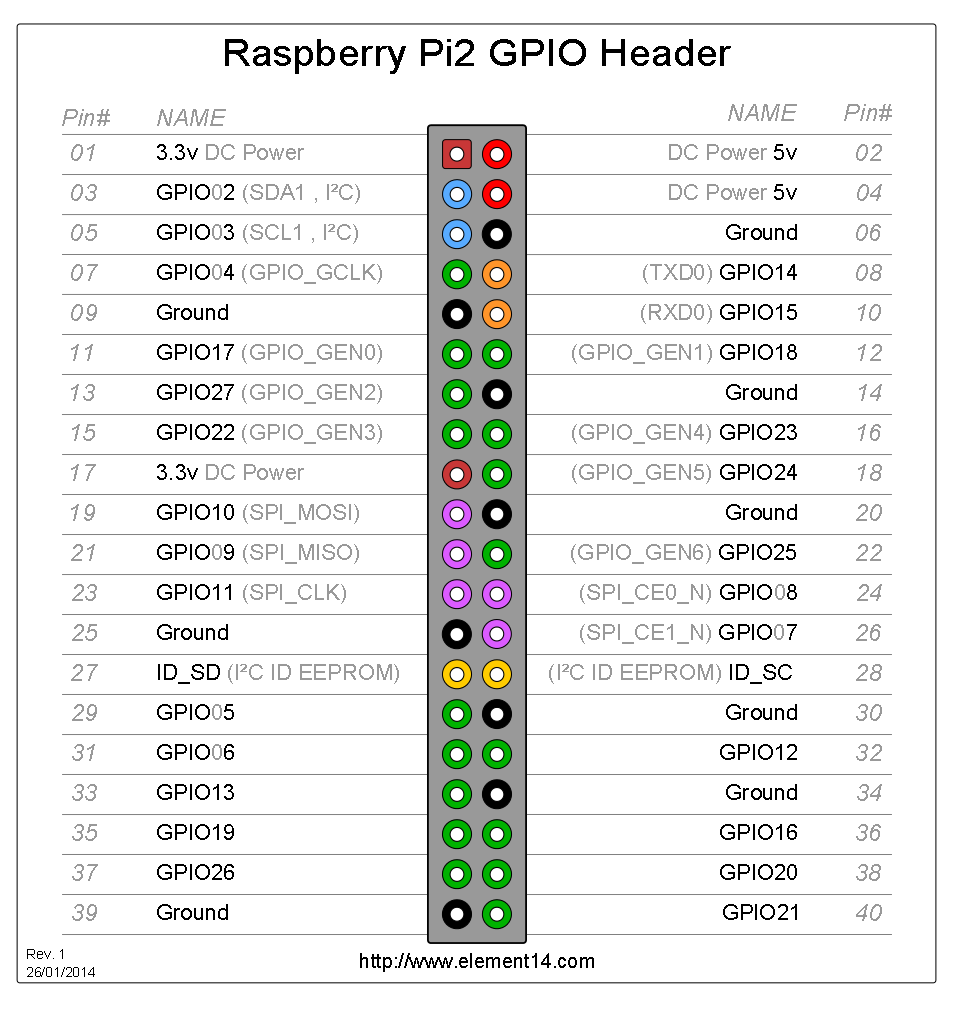
\includegraphics[width=.7\textwidth]{../images/GPIO_Pi2.png}
\end{center}\end{figure}

\Code{Blink the Light.}{code:dbli}{../labs/lab_01/das_blinken_light.py}{Python}

To run the code you need to type the following in the terminal window.

\CommandLine{sudo python \url{das_blinken_light.py}}

You need sudo to give enough permission to access the gpio pins.  The LED should blink on for a sec and off for a sec.

\section{Das Blinken LED II}

\begin{itemize}
  \item all the previous parts
  \item switch
\end{itemize}

Hook up with switch or button to ground.  The Broadcom chip that runs the gpio for the Pi has the ability to connect a pullup or pulldown resistor to an input.  We will thus use a pullup resistor, and the button will pull it down to ground when pressed.

We will now write code to read input and blink led if the button isn't pressed.  Type in:

\CommandLine{sudo nano \url{das_blinken_light_II.py}}

You can also refer to the GitHub repository, if need be.

\Code{Blink the Light while the button is not pressed.}{code:dblii}{../labs/lab_01/das_blinken_light_II.py}{Python}

\CommandLine{sudo python \url{das_blinken_light_II.py}}


\section{Das Blinken LED III}

One last thing for today is to dim the led.  The Raspberry Pi does not have an A/D converter, so we will just deal with two levels based on the button.  We also only have one pulse width modulated output on Broadcom (BCM) pin 18, which is Board pin 12.  Lack of A/D converters is one of several reasons it is not a replacement for a micro-controller, the main one being it doesn't have a real time operating system (RTOS) and lacks the necessary timers, like watchdog timers, to build one.  If you ever need a micro-controller then use an Ardino, MSP430, or similar.  The Pi has a bunch of advantages too in standard tools, quad core, and so on.  We care more about the later for labs and testing.  If you ever build patient used tools, get a micro-controller as you need the RTOS.

Getting back to the point, we want to have the LED on all the time now, and we will dim it when the button is pushed.  To handle the diming, we will use a pulse width modulator.  We will set the frequency to 50Hz, which is a reasonable refresh rate, and will use the duty cycle (percent of the wave that is high) to control the brightness.  This is a simple and standard way to handle this.  Type in:

\CommandLine{sudo nano \url{das_blinken_light_III.py}}

You can also refer to the GitHub repository, if need be.

\Code{Dim the Light while the button is pressed.}{code:dbliii}{../labs/lab_01/das_blinken_light_III.py}{Python}

\CommandLine{sudo python \url{das_blinken_light_III.py}}


\chapter{One Wire Thermometer}

\section{Assemble Circuit}

The basic one wire temperature sensor from Dallas Semiconductor, uses a TO-92 package, just like a transistor.  Originally they only operated in parasitic mode, but the latest versions have had a powered version that can be run in parasitic mode. The pinout is as follows:

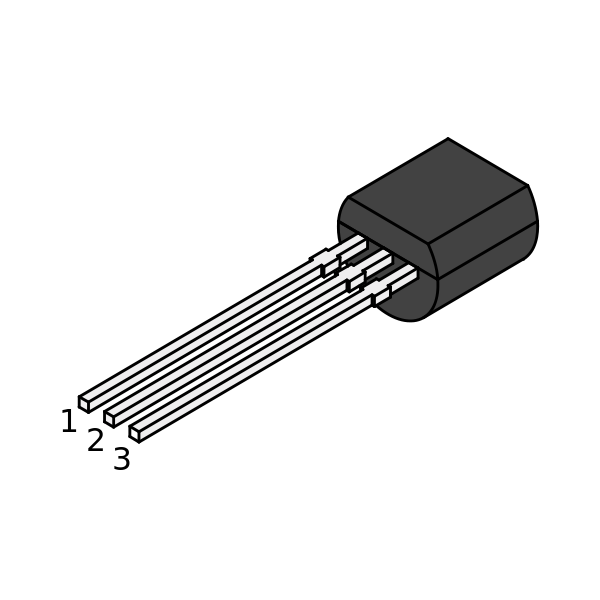
\includegraphics[width=0.4\textwidth]{../images/TO-92-Package.png}

where pin 1 is GND, pin 2 is the data line, and pin 3 is NC on old systems and 3.3v or GND on new ones (Ground for parasitic).  The data line needs a pull-up resistor\footnote{A resistor that supplies power to a bus, connected between the data and 3.3v in our case.} of around 3k$\Omega$ to 6k$\Omega$, with the sugested value at 4.7k$\Omega$. The one wire thermometer is very easy to connect to a Raspberry pi.  Connect pin 1 to ground, pin 2 to GPIO 4 (4th pin on the left of the Raspberry Pi's GPIO), and pin 3 to 3.3 volts.  Now connect a resistor around 4.7k$\Omega$ between pins 2 and 3 of the one wire.  You are ready to set up your Pi!

\section{Add One Wire Support}

First you need to edit the boot configuration file to add one wire support.

\CommandLine{sudo nano /boot/config.txt}

Scroll to the bottom (use the down arrow), then type \textbf{dtoverlay=w1-gpio}.
Save by typing \textbf{ctrl-o} then exit with \textbf{ctrl-x}.

Now reboot to make your changes active.


\CommandLine{sudo reboot}

\section{Test It}


\CommandLine{sudo modprobe w1-gpio}

\CommandLine{sudo modprobe w1-therm}



\CommandLine{cd /sys/bus/w1/devices}

\CommandLine{ls}

Note that the next directory has a really long name, and incorporates the device number so it is not constant on all systems.  This allows multiple to be connected.


\CommandLine{cd 28*}


\CommandLine{cat \url{w1_slave}}

\section{Code It}

\Code{Read from a One Wire Thermometer.}{code:w1}{../labs/lab_04/w1temp.py}{Python} 

%\chapter{Resistive Sensors}


\section{Fast and Cheap}




\Code{Measure resistive sensor by its time constant with 1uf capacitor.}{code:resistmtc}{resistive_measure_time.py}{Python}




\section{Analog to Digital Conversion}



%\appendix

%\chapter{Raspberry Pi Ref}\label{chapter:RPiRef}

\section{Preparing Your Pi}

The Raspberry Pi can use a variety of OS's, but its basic one is a Linux distro.

\begin{description}
  \item[sudo] runs the command after it as another user, who is by default the super user, hence the name Super User DO.
  \item[apt-get] patches and upgrades the system and applications.
\end{description}

sudo apt-get update %get the latest version

sudo apt-get upgrade %upgrade what you have to what you updated

sudo apt-get install git %install git, great way to get lots of code

sudo apt-get install python-dev %install python development

sudo apt-get install python-rpi.gpi %install python raspberry pi gpio tools

\section{getting code}

git clone http://github.com/adafruit/Adafruit-Raspberry-Pi-Python-Code.git

cd Adafruit-Raspberry-Pi-Python-Code

ls

\section{coding}

For Raspberry Pi

The simplest way to ensure some cleanup code gets run is to wrap your while loop in a try/finally block.

If you specifically want to catch Ctrl+C but nothing else, you can use try/except to catch KeyboardInterrupt.

Finally, if you want a more robust way to ensure some cleanup gets done, take a look at lines 312 through 322 in this revision of my Procrastinator's Timeclock utility.

https://github.com/ssokolow/timeclock/blob/3bb9889...

First, it assigns the cleanup function to sys.exitfunc so it'll get called on clean exit, then it hooks all the common POSIX signals the kernel might send s ensure that they trigger a clean exit.

* SIGINT is sent by Ctrl+C, which INTerrupts the program.
* SIGTERM is sent by things like task managers politely asking your program to TERMinate itself.
* SIGHUP is sent by the kernel when your program loses the terminal it's attached to.
* SIGQUIT is sent by Ctrl+\, which asks the program to quit and dump core if core dumping is enabled.

(My code technically doesn't handle SIGQUIT properly, since it doesn't dump core, but I've never seen people using it properly.)

Finally, it also uses try/except to catch Ctrl+C, just to play it safe. (And it's still not perfect because PyGTK doesn't let the program attach a handler for "lost connection to X server")

If you want a version that's a bit more complicated, but also works on Windows, look at this revision:

https://github.com/ssokolow/timeclock/blob/7a50500...

(It checks that each signal exists before hooking it)


\end{document}

